\section{Introduction}
\label{891_1:sec:introduction}

\begin{figure*}
  \centering
  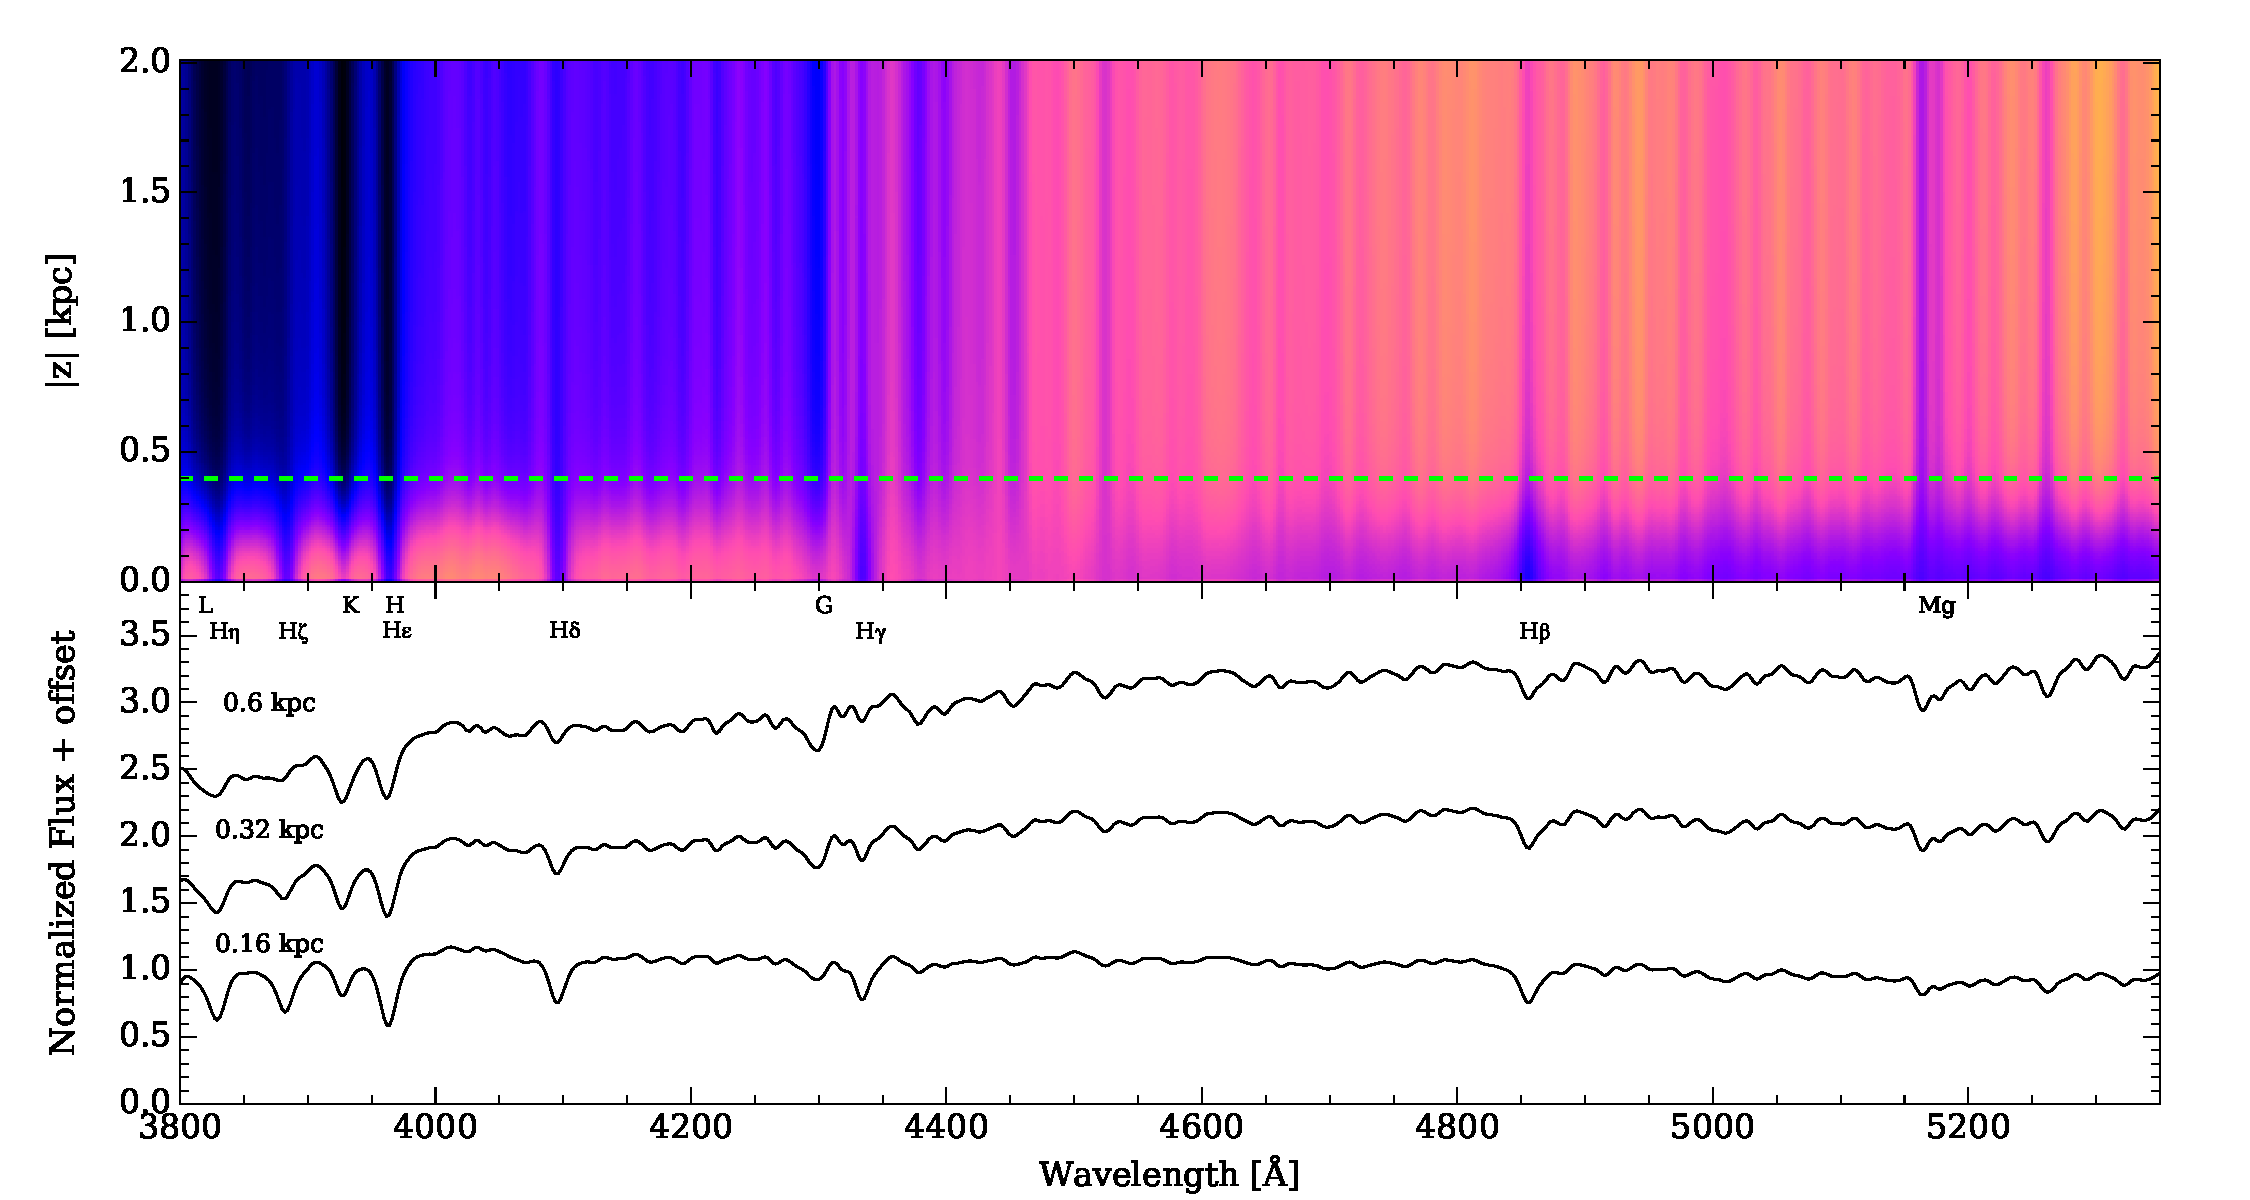
\includegraphics[width=\textwidth]{891_1/figs/mab_stack.pdf}
  \caption[Heating signature in Milky Way
  model]{\label{fig:MW_heating}\fixspacing Example of
    spectrophotometric index change with height and stellar
    population. Spectra are from a model with a fast-rotating (200 km
    s$^{-1}$) disk with a constant star-formation rate and a MW-like
    disk-heating rate, rendered at a spectral resolution of 200 km
    s$^{-1}$ ($\sigma$).  \emph{bottom:} Note the transition from
    Balmer-line to metal-line dominance between 0.32 and
    \val{0.6}{kpc}. \emph{top:} The same model spectra plotted with
    height and color-coded by normalized intensity. The transition
    between Balmer-line and metal-line dominated populations is clear
    in \Hda and Ca H\&K. Our models predict the location of the
    transition is a measure of the disk heating time-scale and is
    largely independent of the details of the star-formation
    history. The green line shows the same transition in NGC 891 at
    \val{0.4}{kpc} as discussed in \S\ref{891_1:sec:results}.}
\end{figure*}

By the middle of the last century it was well established that the
scale-heights and velocity dispersions of stars in the solar
neighborhood increase with age \citep[see][for a summary of this early
  work, particularly the chapters contributed by Elvius and
  Delhaye]{Blaauw65}. The seminal work by \citet{Roman50} demonstrated
that the disk kinematics also depended on metallicity.  Today these
patterns are known in the literature on Galactic archaeology as
age-velocity-metallicity (abundance) relations \citep[AVM$\alpha$-R;
  e.g.,][]{Aumer09,Minchev14}. Observational advances continued for
the solar neighborhood \citep[e.g.,][]{Edvardsson93, Dehnen98,
  Nordstrom04}, and by the beginning of this century the complexity of
these relations have been mapped throughout much of Milky Way (MW) by
wide-field spectroscopic surveys (e.g., RAVE, \citealt{steinmetz06a};
BRAVA, \citealt{howard08a}, SEGUE, \citealt{yanny09a}, LAMOST,
\citealt{zhao12a} GALAH, \citealt{desilva15a},
Gaia-ESO,\citealt{gilmore12a}; and APOGEE-1 and -2,
\citealt{Majewski15}). The radial gradients in these relations are
beautifully shown by, e.g., by \citet{Bovy12c} and \citet{Hayden15},
illustrating both metallicity and abundance as well-known
complementary chemical-evolutionary tracers. Despite a century of
remarkable progress, two broad but intertwined questions remain: (i)
What are the astrophysical processes (i.e., the chemo-dynamical
explanation) leading to the observed relations; and (ii) are these
patterns generic for spiral disks or specific to the Milky Way?

Setting aside chemical evolution for simplicity, there has been a
long-standing debate about the origin of the vertical stratification
of disk stars in phase-space as a function of age (the age-velocity
relation, or AV-R). Historically the argument has been in the context
of dynamical heating from two-body scattering \citep{Spitzer51}, but
the scattering source has been debated \citep[e.g., giant molecular
  clouds, transient spiral structure, or dwarf satellite
  galaxies][]{Spitzer51,Spitzer53,Wielen77,Quinn93,Binney00}, and none
have proven satisfactory to explain the MW's thick disk.  This
framework has been salvaged but also up-ended by relatively recent
evidence for the increasing turbulence (and presumably thickness) of
ionized gas in disks at higher redshift
\citep{Weiner06,Forster-Schreiber09,Wisnioski15}. It seems plausible
that early phases of disk formation involved gas cooling, leaving
behind an old thick-disk stellar component
\citep{Brook04,Bournaud09}. However, thinner relic layers would also
emerge as time progressed \citep{Bird13}, depending critically on the
cooling time-scale for the gas in the presence of star-formation, AGN
feedback, and accretion, but without invoking any need for dynamical
heating. Ironically, this `settling' of the stellar disk with
population age is not unlike the predictions of monolithic collapse
from \citet{ELS}, albeit now consistent in the context of bottom-up,
or hierarchical structure formation as seen in recent simulations
\citep[e.g.,][]{Bird13,Martig14a}.  Because it is no longer clear if,
loosely speaking, disks `heat' or `cool' to form the the vertical
stratification of disk stars in phase-space, and likely both modes
play a role at late and early times, respectively, henceforth we refer
instead to `dynamical stratification' as a phenomenon that captures
both general physical processes.

The recent simulations noted above show there is a rich history of
radial and vertical build up of stellar populations that involves and
interplay between the cooling of the gas, the impact of mergers and
accretion, and at late times the classical heating processes noted
above.  This richness suggests the possibility for a diversity of
astrophysical paths in disk formation that could lead to significantly
different structure in galaxies, exhibited in their
AVM$\alpha$-Rs. Hence, the broader question of whether the MW is
representative of the external disk galaxy population becomes salient.

Little is known about the dynamical stratification rates for stars in
spiral outside the Milky Way, but recent studies of stellar
populations and dynamical stratification in low-mass spiral galaxies
\citep{Seth05a,Bernard15} have shown dramatic differences in the
age-metallicty and age-velocity dispersion relations when compared to
the Milky Way. Recent measurements of the stellar velocity dispersions
in M31 \citep{Dorman15} show that there are also gradients in
dispersion with age and metallicity, but the amplitudes and
time-scales are larger than in the MW. Differences in velocity
dispersion amplitudes may reflect a more massive or thinner M31 disk,
but possibly also a different dynamical history -- for gas settling or
stellar dynamical heating. Clearly more data on the stellar properties
of external galaxies is needed. The above studies serve as a gold
standard since they are based on studies of resolved stellar
populations. Because there are no massive spiral galaxies outside of
the Local Group for which we can resolve stellar populations at
surface-densities high enough to probe most of the disk, it is
imperative to undertake studies based on integrated starlight.

% Underpinning stellar dynamical mass estimates are assumptions about
% the distribution of matter in phase-space. Of importance are the
% density distribution and orbital anisotropy of the luminous tracers
% (Emsellem et al. 2011), both difficult to infer because of geometric
% projection. Typical mass-modeling assumptions include dynamical
% equilibrium, constant $\Upsilon_*$ and orbital anisotropy.  In
% star-forming disks there is every reason to believe these assumptions
% are invalid, even in the vertical direction where luminous young
% stars, gas and dust are in a thin mid-plane layer embedded in
% successively older, thicker, and dynamically warmer stellar
% populations \citep{Mihalas68,Wielen77,Binney00}. Disk components are
% expected to diffuse in a secular fashion through a dynamical heating
% process, forming layers in phase-space. Galaxy disks provide a unique
% laboratory for testing mass-modeling assumptions because they are
% dynamically cold, while on-going star-formation ensures that all
% phases of stellar evolution are present. What is critical is to
% measure the heating rate.

% For the younger and intermediate-age disk components which, for a disk
% like the MW, contains most of the light and a significant amount of
% the stellar disk mass over a modest range of metallicity (and
% therefore plausibly similar IMF). The heating time-scale over the past
% 4-6 Gyr in the solar neighborhood is comparable to the disk radial and
% vertical dynamical time-scales \citep{Aumer09}; even quiescent disks
% are not in true equilibrium. Determining disk heating rates pins down
% vertical gradients in $\Upsilon_*$ to within some {\it constant} scale
% factor (the IMF), thereby enabling a conversion from luminosity to
% {\it relative} density profiles.

% The main thrust of this program is to exploit vertical population
% gradients in star-forming disks to establish disk-heating rates. This
% will provide constraints on the cause(s) of heating, and eliminate
% systematics from our determination of disk gravitational potentials
% and thereby accurately calibrate $\Upsilon_*$. This can be done by
% combining spectroscopic indices that correlate stellar age to their
% kinematics and spatial location: By using integrated starlight as a
% {\it chronometer} it is possible to determine the dynamical evolution
% of disks. Because $\Upsilon_*$ evolves with stellar population age
% independent of uncertainties in the low-mass end of the IMF, such
% measurements decouple IMF uncertainties from the interplay between the
% relative distribution of luminosity and the dynamically-inferred
% mass. In other words, by measuring disk heating rates we will be able
% to distinguish between the mass-weighted scale-height of the disk and
% luminosity-weighted scale-height of our dynamical tracers.  To measure
% disk-heating and apply the results to an accurate mass-decomposition
% of spiral disks our program has this two-step framework:
% 
% \leftskip=0.35in
% {\it                                                                            
%                                                                                 
% \medskip                                                                        
% \noindent (i) determine the vertical age gradients and hence the disk
% heating rate in detail for a small but representative sample of
% $\sim$20 edge-on galaxies; and then
%                                                                                 
% \medskip                                                                        
% \noindent (ii) calibrate a proxy for stellar velocity dispersion
% applicable to large samples of star-forming galaxies at all
% inclinations, and to young stars and old stars. Use this proxy to
% constrain heating rates and dynamical models of stellar disks to infer
% their mass-density.
% 
% }
% \leftskip=0in

\subsection{Experimental Design}

In this paper we present a detailed, spectroscopic study of stellar
populations in the nearby, edge-on galaxy NGC 891 in integrated
starlight mapped over much of the visible stellar disk in both radius
and height. The importance of looking at NGC 891 as well as other
nearby edge-on disks is several fold. First, it allows us to expand
the census of spiral disks beyond the Local Group, particularly for a
geometric projection that allows us to examine the spatial gradients
in both radius and height more directly than in either M31 or the MW.
Second, NGC 891, while historically called out as a nearby MW analog,
clearly has some properties that are exceptional such as a large HI
scale height \citep[$\sim$1 kpc][]{Oosterloo07}, consistent with an
extended dust layer \citep{Howk00}. Measurements of vertical and
radial population gradients in NGC 891 will provide a better picture
of the range of such gradients in MW-like systems, pointing to the
range and multiplicity of disk formation and assembly scenarios of
MW-like galaxies.

As a benchmark for what we might expect to see in terms of
AVM$\alpha$-R in the integrated light of an external, edge-on galaxy,
for illustration purposes we focus again simply on age and velocity
(AV-R, where velocity, i.e., velocity dispersion is rendered in
equivalent height given relevant dynamical assumptions) and ask: If
NGC 891 has a similar star-formation history and AV-R as the MW's
solar cylinder, what would the integrated light look like if observed
edge-on? In answering this question here, our intent is demonstrate
the essence of our experimental design, namely a method to measure
disk dynamical stratification rates by using stars as chronometers.

To estimate the vertical distribution of the stellar spectral energy
distribution we construct a simple model where stars in disks (i) form
at some rate at the mid-plane with a scale-height and velocity
dispersion comparable to the gas; and then (ii) are dynamically
stratified through some secular process over time. We adopt a constant
star-formation rate (SFR) and total age of 11 Gyr\footnote{This is a
  reasonable match for the total age of the MW disk and the
  star-formation formation rate over the past few Gyr based on
  analysis of stars in the solar cylinder
  \citep[e.g.,][]{Pilyugin96a}.}, the `heating' model for the solar
cylinder of \citet{Aumer09}, and we assume the dynamics are such that
$\sigma_z^2/h_z$ is constant at late times, which is roughly what is
observed in the MW disk near the sun ($\sigma_z$ is the vertical
stellar velocity dispersion and $h_z$ is the corresponding
scale-height, i.e., $\sigma_z^2/h_z$ is proportional to the surface
mass-density of the disk). We also adopt the stellar population
synthesis models of \citet{Bruzual03} but note in the spectral range
of interest here the choice is unimportant. By coupling elements (i)
and (ii) to stellar population synthesis models it is them possible to
compute the vertical distribution of star light.

In adopting this simplified model to represent what we might see for
the projected vertical distribution of integrated starlight of an
edge-on galaxy like NGC 891 we are in effect assuming the SFR and
dynamical stratification are constant with radius, which, despite the
apparent radial constancy of disk thickness observed over many radial
scale-lengths in external galaxies, at some level must be
incorrect. Certainly we know there is flaring in gas layers with
radius as well as gradients in the total and specific SFR.  In a
companion paper we discuss details about assumptions of the gas-layer
thickness between NGC 891 and the MW, radial variations in the
gas-layer thickness and heating rate, relative sensitivity to the
star-formation rate versus the heating rate, as well the general
problem of heating models' inability to match the thick disk, as noted
above. The simplifications adopted here allow us to look at what
appear to be the primary observational consequences of dynamical
stratification on vertical trends in the spectral energy distributions
of galaxies; this simple model is likely to capture the interplay of
stellar evolutionary time-scales and dynamical stratification that
dominate the younger and intermediate-age disk components in the MW
\citep{Bird13}.

We illustrate the spectrophotometric rendering of our simple model in
Figure \ref{fig:MW_heating}.  This example shows how the spectra of
integrated star-light would appear as a function of height above the
disk mid-plane for a dynamical stratification rate self-similar to what
is seen in the MW solar cylinder. Inspection shows there is a height
above the disk mid-plane where a rapid transition in the stellar
population occurs at roughly $|z| \sim 0.4$ kpc.  Here, the spectrum
evolves from Balmer-absorption to metal-absorption dominance on the
time-scale of A/F main-sequence stellar lifetimes ($\sim$0.5 Gyr). The
break-height where this occurs is relatively insensitive to
star-formation history, spectroscopic line-strengths are reddening
independent, and line-of-sight attenuation from dust at this expected
break-height is not prohibitive for detection.  Consequently,
measuring the break height yields a constraint on the dynamical
stratification rate on these time-scales. The transition is best
detected in spectra covering the 4000 \AA\ region, and can be
measuring easily even with low-resolution spectrophotometry.

Our first-order objective is to determine if we can detect and measure
a spectral break height in the disk of NGC 891, and if so, how it
compares to the this simple model for the MW solar cylinder. The
height and width over which the spectral break occurs yields a
constraint of AV-R, or the dynamical stratification rate at late
times. While this model may be qualitatively correct for the solar
neighborhood and NGC 891, it is well worth verifying if the observed
gradients are constant with projected radius.  It has been suggested
from the simulations of \citet{Martig14a} that the young, star-forming
disk at every epoch flares), likely for dynamical reasons perhaps
related to the flaring of atomic and molecular gas at the current
epoch. Recent measurements suggest such flaring is seen in MW stars
\citep{Ness16}. We will probe for a similar flaring in NGC 891,
manifest as a change in break height with radius.  While differential
extinction effects cannot be ignored when interpreting line-of-sight
depths of our observations, we will use Doppler tomography in Paper II
\citep[see for example,][]{Kregel05} to increase the fidelity of
our measurements in Paper II.

Our higher-order objective is to probe if the spectrophotometric data
of integrated starlight farther above the mid-plane enables us extend
constraints on the dynamical stratification over longer time frames
commensurate with the old thin and thick disks.  While the
implementation is beyond the scope of the present work, the detection
of metallicity and abundance gradients in both radius and height
provides a mapping of AVM$\alpha$-R in external galaxies, and, via the
appropriate chemo-dynamical model, constraints on the dynamical
stratification for disk stars over most of the star-formation history
of the galaxy.

In this paper we describe the custom fiber integral field unit we
built to make these measurements of vertical population gradients in
nearby, edge-on disks (Section \ref{891_1:sec:pak}).  Our observations of
NGC 891 with this IFU are described in section \ref{891_1:sec:obs}.  The
data reduction and calibration procedures, particularly those specific
to this first variable-pitch IFU, are given in section
\ref{891_1:sec:data_reduction}. The resulting spectral maps are binned based
on signal-to-noise (S/N) criteria motivated by astrophysically
motivated requirements on determining age and metallicity in the
integrated light of stellar populations, and determined via modeling
in Section \ref{891_1:sec:maps}. Spectral diagnostics are measured for these
binned spectra to examine of the trends in age, metallicity and
abundance with radius and height in Section \ref{891_1:sec:results}.  These
give a qualitative picture of the population gradients in this galaxy,
as projected along the line of sight. A synopsis of the results from
this paper are given in Section \ref{891_1:sec:summary}.  In an accompanying
paper we undertake spectral analysis to quantify the line of sight
depth of these observations, and the stellar population gradients in
this galaxy, comparing them to what we might expect in the Milky Way.

% For the younger and intermediate-age disk components which, for a disk
% like the MW, contains most of the light and a significant amount of
% the stellar disk mass over a modest range of metallicity (and
% therefore plausibly similar IMF). The heating time-scale over the past
% 4-6 Gyr in the solar neighborhood is comparable to the disk radial and
% vertical dynamical time-scales \citep{Aumer09}; even quiescent disks
% are not in true equilibrium. Determining disk heating rates pins down

% We use a simple heating model of \citet{Aumer09}, suitable for the MW
% solar cylinder, and based on Hipparcos proper-motion data and
% Geneva-Copenhagen radial velocities. For each cohort of disk stars,
% i.e., those that form at some epoch this yields a vertical velocity
% dispersion that grows as \citep[using the formulation
%   of][]{Wielen77} $$\sigma_z(t) = \sigma_z(0) (1+t/\tau_{\rm
%   heat})^{1/n_h},$$ where $\tau_{\rm heat} \sim 5 \times 10^7$ yr is
% the heating time-scale, $\sigma_z(0)$ is the velocity dispersion of
% the stars at birth, the exponent $n_h$ is referred to as the heating
% index, and time is moving forward from, and indexed to, the cohort
% formation epoch.

% Historically and physically, the model derives from
% \citet{Spitzer51,Spitzer53} molecular-cloud scattering scenario where
% the time-constant for energy transfer for the Solar neighborhood can
% be interpreted in terms of molecular cloud mass and density, the
% initial velocity-dispersion, and a complex function of $B/\omega$
% where $B$ is Oort's constant and $\omega = V_c/R$, i.e., the angular
% velocity. What is relevant here is that the formulation provides a
% simple, analytic model which describes well the phase-space
% stratification of MW disk stars.

% One further required model component relates the vertical thickness to
% velocity dispersion. We assume the dynamics are such
% that $\sigma_z^2/h_z$ is constant at late times, which is roughly what
% is observed in the MW disk near the sun, but that the stellar layer
% never gets thinner or dynamically colder than the gas layer at $h_z =
% 0.065$ kpc and $\sigma_z = 8$ km s$^{-1}$.  While the atomic gas layer
% in NGC 891 is vertically very extended \citep{Swaters97, Oosterloo07},
% the relevant thickness is the molecular gas, which in NGC 891 is much
% thinner, but about a factor of two thicker than the molecular disk in
% the MW \citep{Scoville93, Yim11}. This is a pretty good match to the
% near-infrared ($K$ band) super-thin disk component scale-height of 160
% pc found by \citet{Schechtman-Rook13}. Despite this difference, we
% scale the stellar vertical distribution as a function of their age
% such that they match the MW old thin-disk stars with $h_z = 0.350$
% kpc, $\sigma_z =20$ km s$^{-1}$, and an age of 7 Gyr.

% The specified heating model, however, is parameterized for the solar
% cylinder. In order for the disk to have constant thickness with
% radius, yet a velocity dispersion profile that is roughly exponential
% with twice the photometric scale length - what we observe for disks
% today - at least one of three parameters change with radius: the
% heating time-scale, the heating index, or the initial gas velocity
% dispersion. While any one of these can be modulated with radius to
% achieve a nearly constant vertical scale-height with time and radius,
% it is compelling to keep the heating- index constant (i.e., the
% physical heating mechanism is the same) while setting the heating
% time-scale to be the dynamical time-scale associated with the disk's
% rotation. Note for example that $\tau_{{\rm heat},\odot} \sim (\pi/2)
% R_\odot/V_\odot$ adopting $V_\odot = 220$ km s$^{-1}$ and $R_\odot =
% 8$ kpc as the circular speed and distance to the Galactic center at
% the Solar radius. Except for the inner portion of the galaxy,
% $\tau_{\rm heat}$ is simply a linear function of radius.

% It is also reasonable to adopt an initial velocity dispersion of the
% stars that has a modest trend with radius. This is plausible because
% the gas also exhibits such a trend, as seen by \citet{Shostak84}, and
% more recently updated by \citet{Tamburro09}. We will show elsewhere
% that this produces a time-evolution of a stellar disk that uniformly
% thickens while quickly developing a radial trend in stellar velocity
% dispersion that matches observations in the DMS.

% There is no chemical evolution in the model, but it would be
% straight-forward to add following, e.g.,
% \citet{Pilyugin96a,Pilyugin96b,Chiappini97} based on the earlier
% studies of \citet{Twarog80, Carlberg85,
%   Meusinger91,Edvardsson93}. From these studies, it is reasonable to
% approximate the age-metallicity relation as linear in time with [Fe/H]
% = 0.05 today and [Fe/H] -0.35 8 Gyr ago, then dropping rapidly at
% earlier ages where it would be reasonable to adopt Z = 0.2 solar.

% $h_z(t=7{\rm Gyr})=0.35$ kpc $\sigma_z(t=7{\rm Gyr}) = 20$ km
% s$^{-1}$ Then $\sigma_z(t=0)$ is inferred from $\sigma_z(t=7{\rm
% Gyr})$ using the heating model, but not allowed to be less than
% $sigma_{z,{\rm min}} = \sigma_{\rm gas} / \sqrt{1/a^2+2/3)$ km
% s$^{-1}$, where $a = 0.6$ (why?). The thicknes is given by $h_z(t) =
% h_z(t=7{\rm Gyr})(\sigma_z(t)/\sigma_z(t=7{\rm Gyr}))^2$, with the
% additional imposition that $h_z(t) \geq h_{z,{\rm min}} = 0.065$
% kpc, i.e., the gas layer in the MW, which at least for HI in N891,
% is not a good match. However the relevant thickness is the molecular
% gas, which in NGC 891 is comparable to the MW (Scoville et
% al. 1993).
% 
% For $n_h = 3$, $\tau = 0.05$ Gyr, while for $n_h = 2$, $\tau = 0.2$
% Gyr. These values are from Wielen (1977), but the $n_h = 3$ case is
% consistent with Binney et al. (2000) analysis of Hipparcos data.
% Further, this value of $\tau$ is close to the dynamical time-scale
% $t_{\rm dyn} = 2 \pi R/V$ at the solar circle ($R = 8$ kpc, $V = 220$
% km s$^{-1}$).

% another paper to look at for asymmetry and high-z dust: Hughes et al. 2014

%% \begin{figure}
%%   \centering
%%   \includegraphics[width=\columnwidth]{figs/mab_plot_model.pdf}
%%   \includegraphics[width=\columnwidth]{figs/mab_plot_modelspec.pdf}
%%   \caption{\label{fig:MW_heating}Example of spectrophotometric index change
%%     with height and stellar population. Spectra are from a model with a
%%     fast-rotating (200 km/s) disk with a constant star-formation rate and a
%%     MW-like disk-heating rate. Note the transition from Balmer-line to
%%     metal-line dominance between 0.8 and 1.5 hz. Our models predict the
%%     location of the transition is a measure of the disk heating time-scale and
%%     is largely independent of the details of the star-formation history.}
%% \end{figure}

%% \begin{figure}
%%   \centering
%%   \includegraphics[width=\columnwidth]{figs/mab_plot_model.pdf}
%%   \caption{\label{fig:mab_model}Another view of the spectrophotometric
%%     index change shown in Figure \ref{fig:MW_heating}. Color is mapped
%%     to intensity and all spectra have been normalized to unity mean
%%     over the wavelength interval shown. The horizontal line marks the
%%     age break at \val{0.4}{kpc} found in
%%     \S\ref{891_1:sec:results}. This break is remarkably consistent with the
%%     transition from Balmer-line to metal-line (Ca H\&K) dominance seen
%%     the models.}
%% \end{figure}

 



